%% SECTION HEADER /////////////////////////////////////////////////////////////////////////////////////
\section{Temperature effect on \acl{gw} propagation}
\label{sec:temp}
 
The high propagation velocities of \acp{gw} make a single measurement last up to 2~\unit{\micro\second}.
Compared to slow changes in ambient temperature (in seconds), the propagation phenomenon can be modelled for the stationary temperature field.
It was assumed that the temperature field can be obtained from temperature sensors at the moment of \ac{gw} excitation.
For simplicity, the model assumed a uniform temperature field.

According to \cite{lu2005methodology, kijanka2013gpu}, there are two main factors that influence how temperature affects the Lamb waves propagation. First, the thermal expansion of the plate causes the propagation path to be extended. As the coefficient of thermal expansion of the \ac{cfrp} is relatively low (-0.76 \unit[per-mode = symbol]{\micro\meter\per\kelvin} in longitudinal direction along the reinforcing fibres \cite{ahmed2012study}) it was neglected in the consideration.
The other is the temperature dependence of wave velocity due to the variation in material properties of the components.
In the presented models, only changes in the elastic modulus of \ac{hsc} components were considered, while the density changes were neglected.
The mechanical properties of the considered \ac{hsc} components at the reference temperature \(T_r=20\)\unit{\degreeCelsius} are included in Table~\ref{tab:properties}.
\begin{table}[H]
	\small
	\tabcolsep=0.5cm
	\centering
	\caption{\label{tab:properties}The mechanical properties of the materials at a reference temperature of +20\unit{\degreeCelsius}}
	\begin{tabular}{ccccc}\toprule
		\multirow{2}{*}{\textbf{Material}} & $\boldsymbol{E_{11}}$ & $\boldsymbol{E_{33}}$ & $\boldsymbol{\nu_{12}}$ & $\boldsymbol{\rho}$ \\ & \unit{\giga\pascal} & \unit{\giga\pascal} & -- & \unit[per-mode = symbol]{\kilogram\per\cubic\meter}\\
		\midrule
		Carbon & 275 & 27 & 0.2 & 1900\\
		Epoxy & 3.43 & 3.43 & 0.35 & 1250\\
		Aluminium & 69 & 69 & 0.33 & 2770\\
		Epoxy adhesive & 6 & 6 & 0.34 & 1200\\
		Cyanoacrylate glue & 3 & 3 & 0.34 & 1200\\	
		\ac{pzt} &  59 & 47 & 0.31 & 7850\\
		\bottomrule
	\end{tabular}
\end{table}
Young's modulus for the \ac{cfrp} skin was calculated accordingly to the methodology described in \cite{chamis1983simplified, salamone2009guided, sikdar2018effects}.
The significant changes in mechanical properties under temperature occur mainly in the polymer matrix, while the variation in the carbon fibre properties has a negligible effect on wave propagation.
In this model \cite{salamone2009guided, hopkins2012extreme}, the reduction of Young’s modulus of the resin \(E_m\) with temperature variation was assumed as
\begin{eqnarray}
	E_m(T)=F_m E_{m}(T_r),
	\label{eq:factor_temp}
	\nomtypeR[E]{$E$}{Young's modulus}{}{\unit{\giga\pascal}}%
	\nomtypeR[T]{$T$}{Temperature}{}{\unit{\degreeCelsius}}%
	\nomtypeR[Tr]{$T_r$}{Reference temperature}{}{\unit{\degreeCelsius}}%
\end{eqnarray}
where \(E_{m}(T_r)\) is Young’s modulus of the resin at the reference temperature, and \(F_m\) is the temperature degradation factor.
According to \cite{chamis1983simplified}, it equals
\begin{eqnarray}
F_m=\sqrt{\frac{T_{g0}-T}{T_{g0}-20}},
\nomtypeD[Fm]{$F_m$}{Temperature degradation factor}{}%
\nomtypeR[Tg0]{$T_{g0}$}{Glass transition temperature}{}{\unit{\degreeCelsius}}%
\label{eq:em_temp}
\end{eqnarray}
where \(T_{g0}\) is the glass transition temperature.
Effective temperature-dependent properties of the \ac{cfrp} skin are presented in Figure \ref{fig:cfrpEG}.
The values of Young's modulus along and across carbon fibres, \(E_{11}\) and \(E_{33}\), respectively are depicted in Figure \ref{fig:cfrpEG}(\textbf{a}), and shear modulus \(G_{12}\) and \(G_{23}\) in Figure \ref{fig:cfrpEG}(\textbf{b}).

\begin{figure}
	\begin{center}
		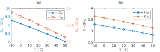
\includegraphics[width=0.95\textwidth]{Chapter_3/cfrpEG}
	\end{center}
	\caption{Temperature-dependent (\textbf{a}) Young's modulus (E\(_{11}\), E\(_{33}\)) and (\textbf{b}) shear modulus (G\(_{12}\), G\(_{23}\)) for the \acs{cfrp} skin}
	\label{fig:cfrpEG}
\end{figure}

Equation (\ref{eq:em_temp}) is also applicable to determine the elastic modulus of the adhesive layer.
The linear temperature dependence for aluminium given by Hopkins~et~al.~\cite{hopkins2012extreme} is defined as
\begin{eqnarray}
	E_a(T)=E_a(T_{r})+\num{4e7}(20-T).
	\label{eq:aluminium_temp}
\end{eqnarray}

Temperature-dependent properties of isotropic materials were determined according to the formulas and the fact that shear and Young's modulus are in relation as \(E=2G(1+\nu)\).
Young's modulus and shear modulus are presented in Figure \ref{fig:isoEG}(\textbf{a}) and Figure \ref{fig:isoEG}(\textbf{b}), respectively, for aluminium, adhesive layer and cyanoacrylate glue.
\begin{figure}[!tbh]
	\begin{center}
		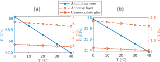
\includegraphics[width=0.95\textwidth]{Chapter_3/isoEG}
	\end{center}
	\caption{Temperature-dependent (\textbf{a}) Young's modulus (E) and (\textbf{b}) shear modulus (G) for isotropic materials used in the simulations}
	\label{fig:isoEG}
\end{figure}

Young's modulus and Poisson's ratio of the sensors were in the form proposed by Lanza et al. \cite{lanza2008temperature}:
\begin{eqnarray}
	\left(E_{11}\right)_{pzt}(T) & = & \left[\left(E_{11}\right)^{-1}_{pzt}(T_r) + \num{2.142857e-14}(20-T)\right]^{-1},\\
	\left(E_{33}\right)_{pzt}(T) & = & \left[\left(E_{33}\right)^{-1}_{pzt}(T_r) + \num{0.777142e-14}(20-T)\right]^{-1},\\
	\nu_{pzt}(T) & = & \nu_{pzt}(T_r) + \num{13e-3}(20-T).
	\label{eq:pzt_temp}
	\nomtypeD[nu]{\( \nu \)}{Poisson's ratio}{}
\end{eqnarray}

The piezo- and electromechanical properties were taken into account based on the
temperature characteristics provided by the manufacturer.
\begin{figure}[!tbh]
	\begin{center}
		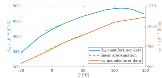
\includegraphics[width=0.95\textwidth]{Chapter_3/pzt_piezo_temp}
	\end{center}
	\caption{Temperature-dependent charge constant (\(d_{33}\)), and electric permittivity (\(\epsilon_{33}\)) of the \acs{pzt} provided by the manufacturer}
	\label{fig:pzt_temp}
\end{figure}
Due to the values provided by the manufacturer being in \(\pm10\%\) tolerance, the characteristics were approximated by the linear functions in the analysed range (see Figure \ref{fig:pzt_temp}) given in the form
\begin{eqnarray}
	\boldsymbol{d}(T) & = & \boldsymbol{d}(T_r) + \left[
	\begin{array}{cccccc}
		0 & 0 & 0 & 0 & 0 & 0\\
		0 & 0 & 0 & 0 & 0 & 0\\
		0.71 & 0.71 & -1.74 & 0 & 0 & 0
	\end{array}\right]\,(20-T) \times10^{-12},\\
	\boldsymbol{\epsilon}^S(T) & = & \boldsymbol{\epsilon}^S(T_r) - \left[
	\begin{array}{ccc}
		3.61 & 0 & 0\\
		0 & 3.61 & 0\\
		0 & 0 & 3.28
	\end{array}\right]\,(20-T) \times10^{-11},\\
	\textbf{e}(T) & = & \boldsymbol{d}(T)\,\textbf{c}_{PZT}(T),
	\label{eq:piezo_temp}
	\nomtypeG{\(\epsilon\)}{Electric permittivity}{}{\unit[per-mode = symbol]
		{\farad\per\metre}}%
	\nomtypeR[d]{\(d\)}{Charge constant}{}{\unit[per-mode = symbol]
		{\coulomb\per\newton}}%
	\nomtypeR[e]{\(e\)}{Piezoelectric coupling coefficient}{}{\unit[per-mode = symbol]
		{\coulomb\per\square\metre}}%
\end{eqnarray}
were \(\boldsymbol{\epsilon}^S\) is the electric permittivity measured at zero strain, \(\boldsymbol{d}\) is the charge constant matrix, \(\boldsymbol{e}\) is the piezoelectric coupling coefficients matrix and \(\boldsymbol{c}_{PZT}\) is the elastic stiffness matrix. 
The manufacturer provided the following piezo constant matrices for reference temperature:
\begin{eqnarray}
	\boldsymbol{d}(T_r) & = & \left[
	\begin{array}{cccccc}
	0 & 0 & 0 & 0 & 669 & 0\\
	0 & 0 & 0 & 669 & 0 & 0\\
	-208 & -208 & 443 & 0 & 0 & 0
	\end{array}\right] \times10^{-12}\ \unit[per-mode = symbol]{\coulomb\per\newton},\\
	\boldsymbol{\epsilon}^S(T_r) & = & \left[
	\begin{array}{ccc}
	802 & 0 & 0\\
	0 & 802 & 0\\
	0 & 0 & 729
\end{array}\right] \times10^{-11}\ \unit[per-mode = symbol]{\farad\per\meter}.
\end{eqnarray}

\begin{figure}[!tbh]
	\begin{center}
		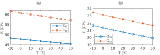
\includegraphics[width=0.95\textwidth]{Chapter_3/pztEG}
	\end{center}
	\caption{Temperature-dependent \textbf{(a)} Young's modulus (E\(_{11}\), E\(_{33}\)) and \textbf{(b)} shear modulus (G\(_{12}\), G\(_{23}\)) for the \acs{pzt}}
	\label{fig:pztEG}
\end{figure}

Temperature-dependent mechanical coefficients for the \ac{pzt} are shown in Figure~\ref{fig:pztEG}(\textbf{a}) for Young's modulus and in Figure~\ref{fig:pztEG}(\textbf{b}) for shear modulus.
For~piezoelectric coupling coefficients (\(e_{31},\ e_{15},\ e_{33}\)) and electric permittivity (\(\epsilon^S_{11},\  \epsilon^S_{33}\)), temperature-dependent characteristics are shown in Figures~\ref{fig:pztEEps}(\textbf{a}) and ~\ref{fig:pztEEps}(\textbf{b}), respectively.


\begin{figure}[!tbh]
	\begin{center}
		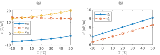
\includegraphics[width=0.95\textwidth]{Chapter_3/pztEEps}
	\end{center}
	\caption{Temperature-dependent (\textbf{a}) piezoelectric coupling coefficients (e\(_{31}\), e\(_{15}\), e\(_{33}\)) and (\textbf{b}) electric permittivity (\(\boldsymbol{\epsilon}^S_{11}\), \(\boldsymbol{\epsilon}^S_{33}\)) for the \acs{pzt}}
	\label{fig:pztEEps}
\end{figure}
\nomtypeG[\(\rho\)]{\( \rho \)}{Mass density}{}{\unit[per-mode = symbol]
	{\kilogram\per\cubic\metre}}
